%%%%%%%%%%%%%%%%%%%%%%%%%%%%%%%%%%%%%%%%%
% Beamer Presentation
% LaTeX Template
% Version 1.0 (10/11/12)
%
% This template has been downloaded from:
% http://www.LaTeXTemplates.com
%
% License:
% CC BY-NC-SA 3.0 (http://creativecommons.org/licenses/by-nc-sa/3.0/)
%
%%%%%%%%%%%%%%%%%%%%%%%%%%%%%%%%%%%%%%%%%

%----------------------------------------------------------------------------------------
%	PACKAGES AND THEMES
%----------------------------------------------------------------------------------------

\documentclass{beamer}
\usepackage{pgfpages}
\usepackage{colortbl}
\usepackage{booktabs}
\usepackage{multirow}
%\pgfpagesuselayout{4 on 1}[a4paper,border shrink=5mm]

\mode<presentation> {

% The Beamer class comes with a number of default slide themes
% which change the colors and layouts of slides. Below this is a list
% of all the themes, uncomment each in turn to see what they look like.

%\usetheme{default}
%\usetheme{AnnArbor}
%\usetheme{Antibes}
%\usetheme{Bergen}
%\usetheme{Berkeley}
%\usetheme{Berlin}
%\usetheme{Boadilla}
%\usetheme{CambridgeUS}
%\usetheme{Copenhagen}
%\usetheme{Darmstadt}
%\usetheme{Dresden}
%\usetheme{Frankfurt}
%\usetheme{Goettingen}
%\usetheme{Hannover}
%\usetheme{Ilmenau}
%\usetheme{JuanLesPins}
%\usetheme{Luebeck}
%\usetheme{Madrid}
%\usetheme{Malmoe}
%\usetheme{Marburg}
%\usetheme{Montpellier}
%\usetheme{PaloAlto}
%\usetheme{Pittsburgh}
%\usetheme{Rochester}
%\usetheme{Singapore}
%\usetheme{Szeged}
\usetheme{Warsaw}

% As well as themes, the Beamer class has a number of color themes
% for any slide theme. Uncomment each of these in turn to see how it
% changes the colors of your current slide theme.

%\usecolortheme{albatross}
%\usecolortheme{beaver}
%\usecolortheme{beetle}
%\usecolortheme{crane}
%\usecolortheme{dolphin}
%\usecolortheme{dove}
%\usecolortheme{fly}
%\usecolortheme{lily}
%\usecolortheme{orchid}
%\usecolortheme{rose}
%\usecolortheme{seagull}
\usecolortheme{seahorse}
%\usecolortheme{spruce}
%\usecolortheme{whale}
%\usecolortheme{wolverine}

%\setbeamertemplate{footline} % To remove the footer line in all slides uncomment this line
%\setbeamertemplate{footline}[page number] % To replace the footer line in all slides with a simple slide count uncomment this line

%\setbeamertemplate{navigation symbols}{} % To remove the navigation symbols from the bottom of all slides uncomment this line
}

\usepackage{graphicx} % Allows including images
\usepackage{booktabs} % Allows the use of \toprule, \midrule and \bottomrule in tables
\usepackage{array}
\usepackage{xcolor}
\usepackage{tabu}
\usepackage{textpos}
\usepackage{animate}
\usepackage{hyperref}
\usepackage{bm}

\pdfpageattr {/Group << /S /Transparency /I true /CS /DeviceRGB>>}
\definecolor{links}{HTML}{2A1B81}
\hypersetup{colorlinks,linkcolor=,urlcolor=links}

\addtobeamertemplate{frametitle}{}{%
\begin{textblock*}{100mm}(.9\textwidth,-0.75cm)
\includegraphics[height=0.7cm, trim=0cm 3.9cm 0cm 0cm, clip=true]{U:/Misc/Logos/LICTR_logo}
\end{textblock*}}



%----------------------------------------------------------------------------------------
% Presentation for RSS meeting, 30 mins, covering SMMR paper
%----------------------------------------------------------------------------------------

%----------------------------------------------------------------------------------------
%	TITLE PAGE
%----------------------------------------------------------------------------------------

\title{MDG: Estimating ICCs in pilot trials} 

\author{Duncan T. Wilson}
\institute[LICTR] % Your institution as it will appear on the bottom of every slide, may be shorthand to save space
{
\includegraphics[height=0.7cm, trim=0cm 3.9cm 0cm 0cm, clip=true]{U:/Misc/Logos/LICTR_logo}\\
Clinical Trials Research Unit \\ % Your institution for the title page
Leeds Institute of Clinical Trials Research \\
University of Leeds \\
\medskip
\textit{d.t.wilson@leeds.ac.uk} % Your email address
}
\date{25th October 2016} % Date, can be changed to a custom date

\begin{document}

\begin{frame}
\titlepage % Print the title page as the first slide
\end{frame}

\begin{frame}
\frametitle{Overview}
\tableofcontents 
\end{frame}

%----------------------------------------------------------------------------------------
%	PRESENTATION SLIDES
%----------------------------------------------------------------------------------------

\section{Background}

\begin{frame}
\frametitle{}

Suppose we want to design (i.e. choose sample size) of a phase III cluster randomised trial. We have the usual formula
\begin{equation}
n = 2 \frac{\sigma^{2}}{\delta^{2}}(z_{1-\beta} - z_{\alpha.2})^{2}[1+(m-1)\rho],
\end{equation}
where $\rho$ is the ICC, $m$ is the cluster size, and $[1+(m-1)\rho]$ is known as the \emph{design effect}. Equivalently, the power of a trial is given by
\begin{equation}
1-\beta = \Phi\left( \sqrt{ \frac{n\delta^{2}}{2\sigma^{2}[1+(m-1)\rho]} } + z_{\alpha/2} \right)
\end{equation}
\end{frame}

\begin{frame}
\frametitle{}
\begin{equation}
1-\beta = \Phi\left( \sqrt{ \frac{n\delta^{2}}{2\sigma^{2}[1+(m-1)\rho]} } + z_{\alpha/2} \right)
\end{equation}
\begin{itemize}
\item Suppose we know $\sigma^{2}$, the total variance. How sensitive is power to the true value of the ICC $\rho$? 
\item Going further: given a distribution for $\rho$, what will the distribution of power look like?
\end{itemize}
\end{frame}

\begin{frame}
\frametitle{}
\begin{thebibliography}{99}
\bibitem{Spiegelhalter2001} David J. Spiegelhalter (2001) 
\newblock Bayesian methods for cluster randomized trials with continuous responses
\newblock \emph{Statistics in Medicine}, 20, 435-452.
\end{thebibliography}
\end{frame}

\begin{frame}
\frametitle{}
\begin{itemize}
\item So, important to have a good estimate of $\rho$ to design the trial.
\item How to get a good estimate?
\item Through an external pilot?
\item E.g. TIGA-CUB, `an investigation of the clustering effect (ICC) relating to the Child Psychotherapists will be carried out to aid sample size calculation'.
\end{itemize}
\end{frame}

\begin{frame}
\frametitle{}
\begin{thebibliography}{99}
\bibitem{Eldridge2015} Sandra M. Eldridge et al. (2015) 
\newblock How big should the pilot study for my cluster randomised trial be?
\newblock \emph{Statistical Methods in Medical Research}, 25, 1039-1056.
\end{thebibliography}
\end{frame}

\begin{frame}
\frametitle{}
\begin{itemize}
\item Conclusion: pilot studies aren't big enough to generate reliable ICC estimates.
\item Instead, we should build estimates from a number of other sources, e.g. other trials, observational studies, papers publishing big lists of ICC estimates, \ldots
\item Makes sense - but how? Meta analyses, evidence synthesis?
\item However we do it, is it going to be much more work to define a prior distribution rather than a point estimate?
\item If we have a prior, should we still ignore pilot data?
\item If we don't want to ignore pilot data, how should we choose its sample size?
\end{itemize}
\end{frame}

\section{Methods}

\begin{frame}
\frametitle{}
Suppose we have an (informative) prior distribution $p(\rho)$ for our ICC, e.g. $\rho \sim Beta(1.5, 10)$. 
\pause
If we conduct our pilot trial and observe $x$, we can get the posterior distribution for $\rho$ using Bayes' rule:
\begin{equation}
p(\rho \mid x) = \frac{p(x \mid \rho) p(\rho)}{p(x)}.
\end{equation}
Now, how do we use this to choose the sample size of the main trial? We can follow Spiegelhalter (and others) and ask that the trial is going to be powered (say, at 90\%) with at least a certain probability (say, 0.8).
\end{frame}

\begin{frame}
\frametitle{}
So, after the pilot trial gives us $x$, we choose the smallest $k$ such that
\begin{equation}
\int_{0}^{1} f(\rho, k)p(\rho \mid x) d\rho \geq 0.8,
\end{equation}
where $f(\rho, k)$ is an indicator function which returns 1 if a trial of $k$ clusters and an ICC of $\rho$ is powered, and 0 otherwise.
\end{frame}

\begin{frame}
\frametitle{}
Before the pilot trial, $x$ is unknown. We want to derive the joint predictive distribution of the main trial's sample size and its power. We can generate samples:
\begin{enumerate}
\item Sample $x_{i}, \rho_{i}$ from $p(x, \rho) = p(x \mid \rho) p(\rho)$
\item Use $x_{i}$ to get the associated main trial sample size $k_{i}$ as above
\item Calculate the power of the main trial, $1-\beta_{i}$ using the earlier formula and the sampled $\rho_{i}$
\item Do this to generate lots of $k_{i}, 1-\beta_{i}$ pairs
\end{enumerate}
\end{frame}

\begin{frame}
\frametitle{}
Compare with two other ways to choose the main trial $k$:
\begin{enumerate}
\item As in Eldridge et al., use the pilot data to compute an estimate $\hat{\rho}$ and plug this into the usual formula;
\item Ignore the pilot data and use only your prior knowledge to form a point estimate $\hat{\rho}$, e.g. choosing the mean /  median / mode of the prior, then plug into the usual formula.
\end{enumerate}
Compare with other pilot sample sizes $k_{p}$.
\end{frame}

\section{Experiments}

\begin{frame}
\frametitle{}
As a \emph{very} tentative first step, a quick implementation lets us look at the joint predictive distribution of the main trial sample size $k$ and its power.
\begin{itemize}
\item Pilot sample size is $k_{p} = 10$.
\item Cluster size in both trials is fixed at $m = 10$.
\item In the main trial we want to detect a standardised effect size of $\delta/\sigma = 0.3$ with a power of 0.9.
\item We take 500 samples of the joint distribution for $k, 1-\beta$.
\end{itemize}
\end{frame}

\begin{frame}
\frametitle{}
\begin{tabular}{c c c c}
\toprule
 & Bayesian & Using pilot & Ignoring pilot \\
\midrule
Prob underpowered 	& 0.18 & 0.51 & 0.39 \\
Mean power			& 0.94 & 0.87 & 0.89 \\
Mean $k$			& 62 & 54 & 51 \\
\bottomrule
\end{tabular}
\end{frame}

\begin{frame}
\frametitle{}
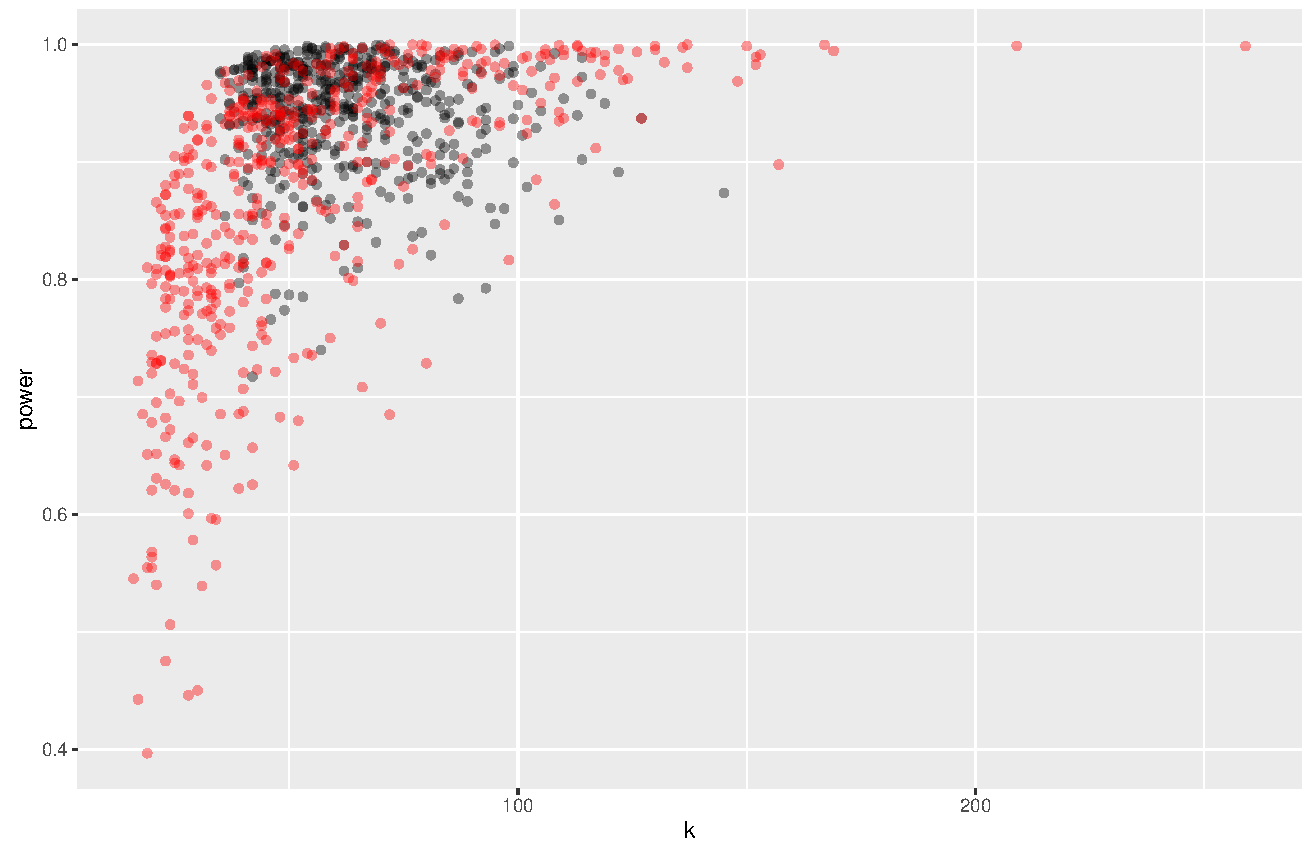
\includegraphics[scale=0.5]{./1vs2.pdf}
\end{frame}

\begin{frame}
\frametitle{}
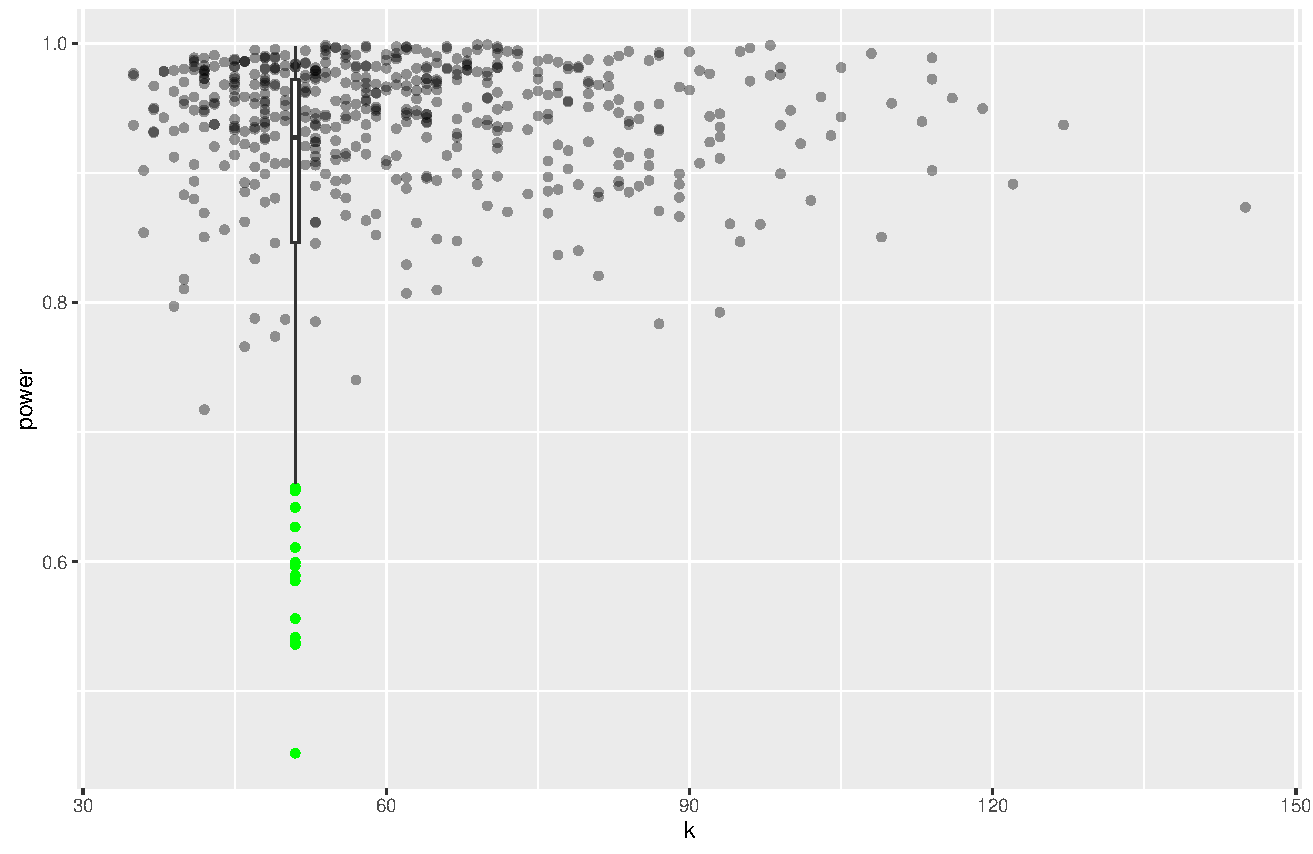
\includegraphics[scale=0.5]{./1vs3.pdf}
\end{frame}

\begin{frame}
\frametitle{}
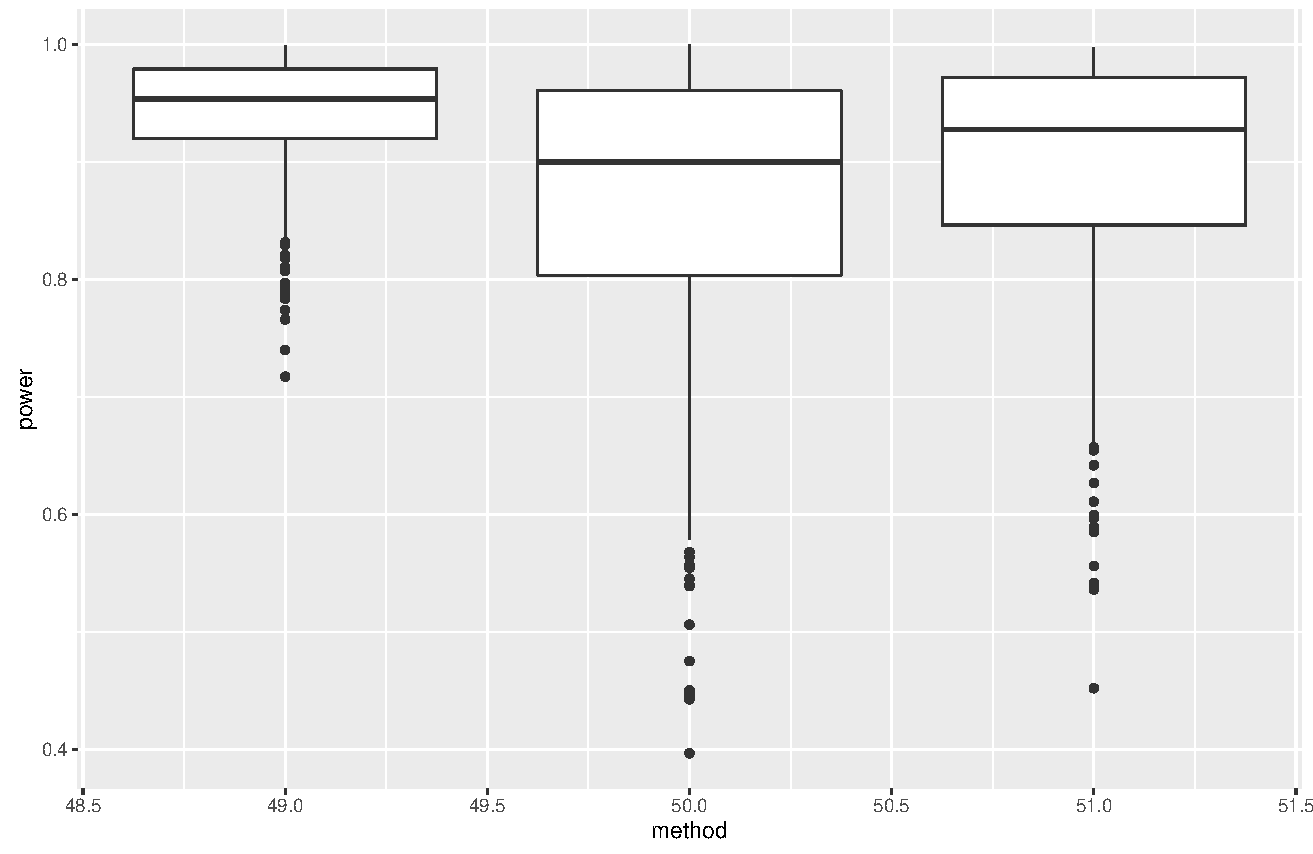
\includegraphics[scale=0.5]{./power_box}
\end{frame}

\begin{frame}
\frametitle{}
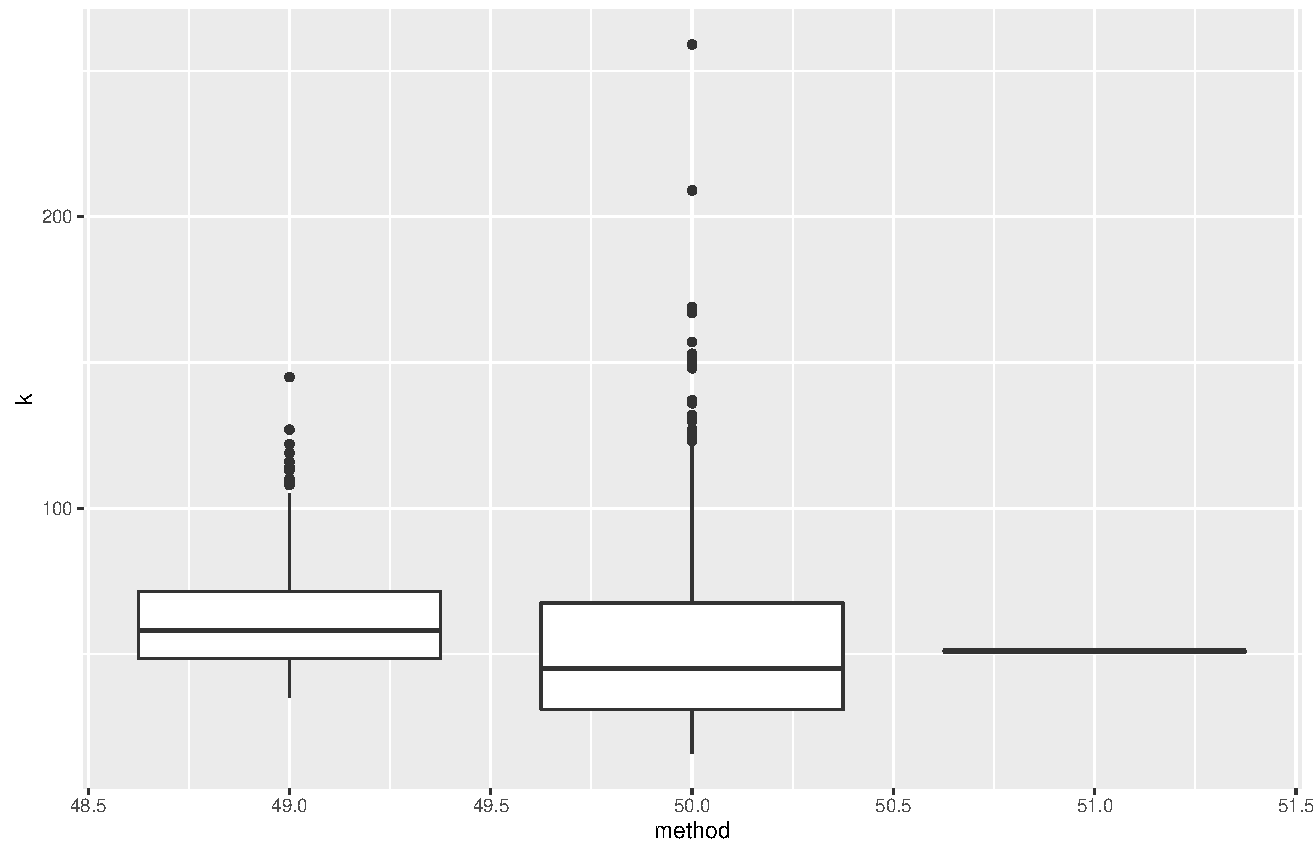
\includegraphics[scale=0.5]{./k_box}
\end{frame}

\begin{frame}
\frametitle{}
Comparisons are between joint distributions on $(k_{p} + k, \beta)$ - how to decide which is better?
\end{frame}

\section{Next steps}

\begin{frame}
\frametitle{}
Defining scope and questions to answer:
\begin{itemize}
\item Only uncertainty in the ICC, or in both variance components?
\item Only cluster randomised trials, or all nested or partially nested designs?
\item When will the different methods be better than each other?
\item When will full elicitation be worthwhile?
\item When will a pilot trial be worthwhile (purely as a means of ICC estimation)? When would it be better to try and elicit a less variable prior?
\end{itemize}
\end{frame}

\begin{frame}
\frametitle{}
Making the computations feasible:
\begin{itemize}
\item Currently we optimise $k$ for the main trial, and for each optimisation iteration we integrate over $p(\rho \mid x)$.
\item We then need to do this many times using different samples of $p(x, \rho)$ for some pilot sample size $k_{p}$.
\item We then want to optimise over $k_{p}$.
\item Similar to decision-theoretic sample size determination - Lindley 1997.
\end{itemize}
\end{frame}

\begin{frame}
\frametitle{}
Extending to other cases:
\begin{itemize}
\item Estimating several nuisance parameters? Multivariate prior elicitation?
\item Incorporating uncertainty in the effect size?
\item Likelihood function not available? Approximate Bayesian Computation (ABC)?
\end{itemize}
\end{frame}


\end{document}





